\documentclass[10pt,a4paper]{article}

\usepackage[a4paper,margin=22mm,headheight=14pt,footskip=12mm]{geometry}
\usepackage[T1]{fontenc}
\usepackage{lmodern}
\usepackage{microtype}
\usepackage{graphicx}
\usepackage{booktabs}
\usepackage{tabularx}
\usepackage{array}
\usepackage{longtable}
\usepackage{enumitem}
\usepackage{xcolor}
\usepackage{amsmath}
\usepackage{fancyhdr}
\usepackage[hidelinks]{hyperref}

\definecolor{ink}{HTML}{20252B}
\definecolor{muted}{HTML}{5F6872}
\definecolor{rule}{HTML}{D9DEE4}
\definecolor{linkblue}{HTML}{175A86}
\definecolor{lightgray}{HTML}{F4F6F8}

\hypersetup{
  colorlinks=true,
  linkcolor=linkblue,
  urlcolor=linkblue,
  citecolor=linkblue,
  pdftitle={Pulse: Customer Journey, Experiment, and Targeting Economics},
  pdfauthor={Pulse},
  pdfsubject={Synthetic digital-banking analytics case study}
}
\graphicspath{{artifacts/figures/}{../artifacts/figures/}}
% Generated by scripts/build_latex_inputs.py. Do not edit this file.
\newcommand{\DatasetCustomers}{100,000}
\newcommand{\DatasetStart}{2025-01-01}
\newcommand{\DatasetEnd}{2026-01-25}
\newcommand{\ActivationContract}{Funded and at least one settled meaningful transaction in signup calendar days 0-7 inclusive.}
\newcommand{\OverallDThirty}{23.604\%}
\newcommand{\SustainedDThirty}{20.909\%}
\newcommand{\DThirtyCount}{23,604}
\newcommand{\SustainedDThirtyCount}{20,909}
\newcommand{\DSevenMature}{29.7\%}
\newcommand{\DThirtyMature}{23.6\%}
\newcommand{\DSixtyMature}{20.5\%}
\newcommand{\DNinetyMature}{16.3\%}
\newcommand{\JuneDThirty}{19.18\%}
\newcommand{\JuneDSixty}{20.02\%}
\newcommand{\ControlN}{18,647}
\newcommand{\TreatmentN}{18,693}
\newcommand{\ControlRate}{69.64\%}
\newcommand{\TreatmentRate}{78.80\%}
\newcommand{\RiskDifference}{+9.16 pp}
\newcommand{\RiskCI}{+8.28 pp to +10.05 pp}
\newcommand{\ExperimentPValue}{$p < 0.001$}
\newcommand{\ExperimentMDE}{+1.33 pp}
\newcommand{\CampaignDiD}{+1.03 pp}
\newcommand{\CampaignIPTW}{+0.95 pp}
\newcommand{\CampaignIPTWCI}{+0.09 pp to +1.80 pp}
\newcommand{\CampaignSE}{0.0044}
\newcommand{\CampaignESS}{42,116}
\newcommand{\CampaignComparisonN}{21,275}
\newcommand{\CampaignTreatmentN}{28,540}
\newcommand{\CommonSupport}{100.0\%}
\newcommand{\WeightedMaxSMD}{0.00349}
\newcommand{\SelectedModel}{regularized logistic}
\newcommand{\SelectionRule}{Regularized logistic is fixed as the selected operational model for interpretability; the comparison table remains the evaluation record.}
\newcommand{\ChurnAUC}{0.752}
\newcommand{\ChurnLift}{2.673}
\newcommand{\ChurnCapture}{26.7\%}
\newcommand{\ChurnEvaluationN}{11,728}
\newcommand{\ChurnTopDecileN}{1,173}
\newcommand{\ResponseAUC}{0.607}
\newcommand{\ResponseLift}{1.160}
\newcommand{\ResponseCapture}{11.6\%}
\newcommand{\ResponseEvaluationN}{4,635}
\newcommand{\ResponseTopDecileN}{464}
\newcommand{\MaxPSI}{0.0023}
\newcommand{\BestStrategy}{expected value}
\newcommand{\EvaluatedPopulation}{11,728}
\newcommand{\ExpectedNetValue}{0}
\newcommand{\TreatmentEffectAssumption}{12.0\%}
\newcommand{\ContactCost}{0.25}
\newcommand{\IncentiveCost}{0.50}
\newcommand{\CapacityFraction}{10\%}
\newcommand{\JourneyRows}{signup & 100,000 & 100.0\% & 100.0\% \\
onboarding completed & 74,458 & 74.5\% & 74.5\% \\
account funded & 58,078 & 58.1\% & 78.0\% \\
first transaction 7d & 42,254 & 42.3\% & 72.8\% \\
repeat usage & 40,996 & 41.0\% & 97.0\% \\
sustained engagement d30 & 20,909 & 20.9\% & 51.0\% \\}
\newcommand{\ExperimentRows}{Control & 18,647 & 12,985 & 69.6\% & 39.6\% & 34.5\% \\
Treatment & 18,693 & 14,730 & 78.8\% & 42.7\% & 39.0\% \\}
\newcommand{\GuardrailRows}{sample ratio mismatch & 0.501 & 0.020 & pass \\
max absolute smd & 0.023 & 0.100 & pass \\
support contact rate difference & 0.019 & 0.050 & pass \\
failed payment rate difference & -0.005 & 0.030 & pass \\
incentive cost per customer & 0.350 & 0.500 & pass \\}
\newcommand{\PretrendRows}{-4 & 22.8\% & 23.4\% & +0.64 pp \\
-3 & 22.0\% & 22.3\% & +0.27 pp \\
-2 & 21.0\% & 21.1\% & +0.03 pp \\
-1 & 20.1\% & 20.6\% & +0.46 pp \\
0 & 20.1\% & 21.1\% & +0.98 pp \\
1 & 18.2\% & 19.7\% & +1.43 pp \\
2 & 17.2\% & 18.8\% & +1.55 pp \\
3 & 16.6\% & 18.2\% & +1.59 pp \\}
\newcommand{\ModelRows}{rule baseline & 0.158 & 0.500 & 0.196 & 0.995 & 10.0\% \\
regularized logistic & 0.133 & 0.752 & 0.439 & 2.673 & 26.7\% \\
hist gradient boosting & 0.133 & 0.750 & 0.435 & 2.669 & 26.7\% \\}
\newcommand{\MonitoringRows}{2025-08-01 & 1,668 & 15.8\% & 0.761 & 3.405 & 0.024 \\
2025-09-01 & 5,318 & 21.5\% & 0.738 & 2.477 & 0.002 \\
2025-10-01 & 4,742 & 18.8\% & 0.761 & 2.793 & 0.015 \\}
\newcommand{\EconomicsRows}{contact all & 11,728 & 100.0\% & -8,567 & No \\
risk & 1,172 & 10.0\% & -815 & No \\
value & 1,172 & 10.0\% & -859 & No \\
response & 1,172 & 10.0\% & -855 & No \\
expected value & 0 & 0.0\% & 0 & No \\}
\newcommand{\BankRows}{State Bank of India & FY2025 & YONO had 8.8 crore registered users, up from 7.4 crore in March 2024; retail internet banking had 13.9 crore customers. & Model multiple digital channels and changing adoption mixes. \\
Axis Bank & FY2025 & Mobile banking had about 3 crore registered customers and more than 15 million monthly active users; the open platform covered 30+ products. & Separate registration, monthly activity, and product depth. \\
HDFC Bank & FY2025 & The bank reported 3.7 crore+ monthly customer engagements on HDFC Bank One, 97\% of financial transactions through digital channels, and 19.3 lakh merchants onboarded to SmartHub Vyapar. & Use heterogeneous retail and merchant activity intensity. \\
ICICI Bank & February 2024 & iMobile had onboarded more than one crore customers of other banks, with repeat use across payments, transfers, recharges, and balance checks. & Include non-primary users and product-specific repeat behaviour. \\
Kotak Mahindra Bank & FY2025 & A regulatory direction paused digital onboarding and new credit-card issuance until February 2025 while the bank deepened existing 811 relationships and reworked its persona-based app strategy. & Include cohort-level acquisition shocks and reactivation. \\}


\setlength{\parindent}{0pt}
\setlength{\parskip}{5pt}
\emergencystretch=2em
\setlist{nosep,leftmargin=17pt}
\setlist[itemize]{topsep=2pt}
\renewcommand{\arraystretch}{1.18}
\newcolumntype{Y}{>{\raggedright\arraybackslash}X}
\newcolumntype{L}[1]{>{\raggedright\arraybackslash}p{#1}}

\pagestyle{fancy}
\fancyhf{}
\fancyhead[L]{\small Pulse analytics report}
\fancyhead[R]{\small Synthetic evidence}
\fancyfoot[C]{\small\thepage}
\renewcommand{\headrulewidth}{0.3pt}
\renewcommand{\footrulewidth}{0pt}

\newcommand{\source}[1]{\par\vspace{1pt}{\footnotesize Evidence: #1.}}
\newcommand{\claim}[1]{\textbf{Claim boundary.} #1}
\newcommand{\tightcaption}[1]{\caption{\small #1}}

\begin{document}

\begin{titlepage}
\thispagestyle{empty}
\vspace*{13mm}
{\Large\bfseries Pulse}\par
\vspace{4mm}
{\huge\bfseries Customer journey, experiment,\par target selection, and economic decision}\par
\vspace{7mm}
{\large A formal report from a reproducible synthetic digital-banking analytics run}\par
\vspace{18mm}
\begin{tabularx}{\textwidth}{@{}L{35mm}Y@{}}
Population & \DatasetCustomers{} synthetic customers.\\
Observation period & \DatasetStart{} through \DatasetEnd{}.\\
Primary decision & Continue controlled activation testing. Do not launch positive-contact outreach under the stated scenario assumptions.\\
Evidence classes & Synthetic descriptive metrics; randomized intent-to-treat estimate; observational DiD and IPTW diagnostics; temporal predictive evaluation; scenario economics.\\
\end{tabularx}
\vfill
\rule{\textwidth}{0.4pt}\par
\vspace{3mm}
\small This report reads generated artifacts. It does not claim production performance, customer impact, or deployment readiness. Numerical statements use the denominators and claim scopes recorded in the artifacts.
\end{titlepage}

\tableofcontents
\clearpage

\section{Executive summary and decision}

Pulse is a synthetic, deterministic customer-analytics case study. It links a customer journey, cohort retention, an activation experiment, an observational campaign analysis, churn and response models, monitoring outputs, and targeting economics. The analysis does not use customer data.

The primary decision is narrow. Continue the activation intervention as a controlled experiment because the randomized estimate is positive and precise for the stated eligible population. Do not launch a positive-contact campaign under the supplied fictional value and cost assumptions: every positive-contact strategy has negative expected net value, while the expected-value policy contacts no customers.

\begin{table}[!htbp]
\centering
\caption{Decision-relevant results from the frozen full run.}
\begin{tabularx}{\textwidth}{@{}L{42mm}Y@{}}
\toprule
Evidence & Recorded result and interpretation \\
\midrule
Journey & Overall D30 retention is \OverallDThirty{} (\DThirtyCount{} customers). Sustained sequential D30 engagement is \SustainedDThirty{} (\SustainedDThirtyCount{} customers). These are different metrics. \\
Randomized experiment & Treatment minus control first-week activation risk difference is \RiskDifference{}; the 95\% confidence interval is \RiskCI{}; \ExperimentPValue{}. \\
Observational campaign & Unweighted DiD is \CampaignDiD{}. Stabilized IPTW DiD is \CampaignIPTW{} with 95\% interval \CampaignIPTWCI{}. Diagnostics do not validate a causal effect. \\
Prediction & The selected \SelectedModel{} churn model records ROC AUC \ChurnAUC{} and top-decile lift \ChurnLift{} on a later temporal holdout. This is predictive association, not treatment benefit. \\
Economics & The best recorded policy is ``\BestStrategy.'' Its expected net value is \ExpectedNetValue{} fictional units after evaluating \EvaluatedPopulation{} customers. \\
\bottomrule
\end{tabularx}
\end{table}

The report separates verified facts from interpretation. All metrics in this section come from \path{artifacts/results.json} and its linked tables. The decision is an interpretation conditional on those metrics, the synthetic data-generating process, and the documented assumptions.

\section{Synthetic-data scope and metric contract}

The full run contains \DatasetCustomers{} synthetic customers from \DatasetStart{} through \DatasetEnd{}. The simulation includes onboarding, funding, meaningful transactions, product activity, cohort changes, a campaign, experiment eligibility, and subsequent outcomes. Public Indian-bank disclosures inform lifecycle structure only; they do not calibrate the numerical retention rates.

The canonical activation definition is: \emph{\ActivationContract}. A meaningful transaction is a settled, non-negative transaction whose type is \texttt{card\_transaction}, \texttt{transfer}, or \texttt{bill\_payment}. Retention uses day windows: D7 is days 7--13, D30 is days 30--36, D60 is days 60--66, and D90 is days 90--96. A funnel row uses the immediately preceding stage as its denominator unless it is labelled as a signup conversion.

\begin{table}[!htbp]
\centering
\caption{Sequential journey counts and denominators.}
\small
\begin{tabularx}{\textwidth}{@{}L{42mm}r r r@{}}
\toprule
Stage & Customers & Signup conversion & Previous-stage conversion \\
\midrule
\JourneyRows
\bottomrule
\end{tabularx}
\end{table}

\begin{figure}[!htbp]
\centering
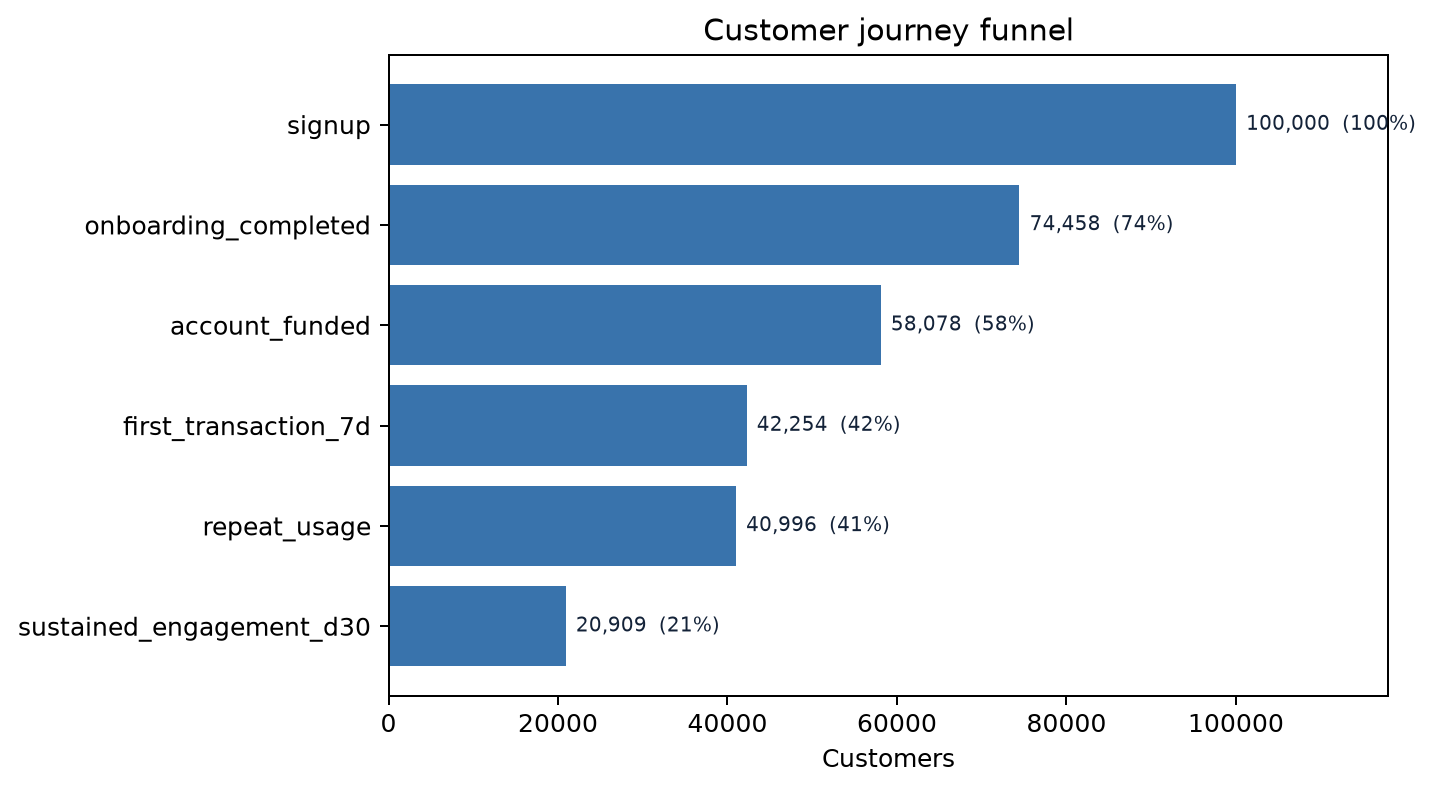
\includegraphics[width=0.86\textwidth]{journey_funnel.png}
\tightcaption{Journey funnel from the generated table. The sustained sequential D30 row is not the same denominator as overall D30 retention.}
\end{figure}

\source{\path{artifacts/results.json}, \path{artifacts/tables/journey.csv}, \path{config/metrics.yml}, and \path{docs/metric_definitions.md}}

\section{Journey and cohorts}

The early journey narrows from signup to onboarding, funding, and first meaningful transaction. The first transaction in the signup-week window is the activation outcome used in the randomized experiment. Repeat usage is a sequential stage. Sustained D30 engagement is a stricter sequential condition than overall D30 retention, which is measured directly against signup.

The mature-cohort estimates decline from \DSevenMature{} at D7 to \DThirtyMature{} at D30, \DSixtyMature{} at D60, and \DNinetyMature{} at D90. The cohort table stores maturity windows and the analysis cutoff, so recent cohorts are not silently treated as inactive.

\begin{figure}[!htbp]
\centering
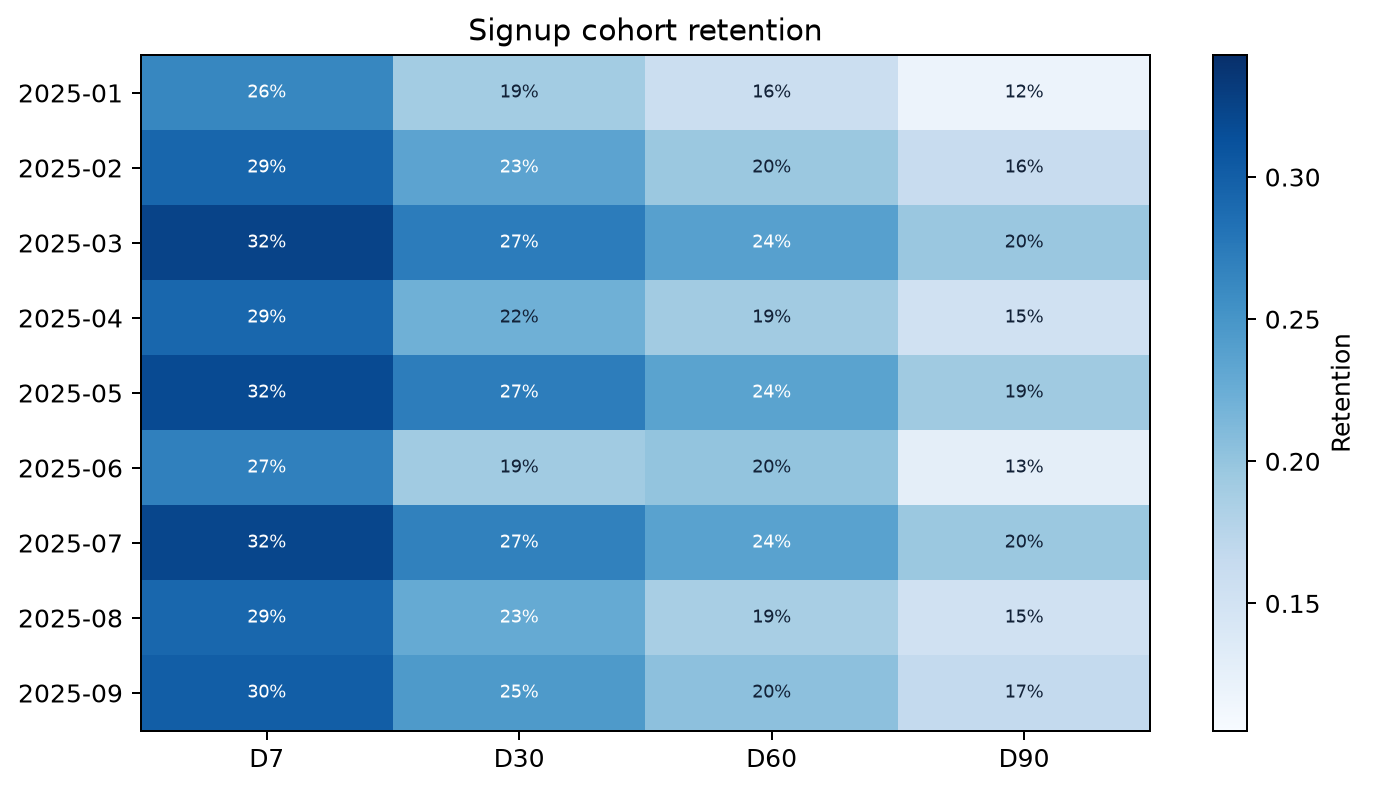
\includegraphics[width=0.88\textwidth]{cohort_retention.png}
\tightcaption{Retention by signup cohort and observation horizon. The plotted values are descriptive synthetic cohort estimates.}
\end{figure}

The June 2025 cohort shows a reactivation bump from its D30 window to its D60 window: the table records \JuneDThirty{} at D30 and \JuneDSixty{} at D60. This increase is compatible with later activity after an earlier inactive window. It does not establish why the bump occurred.

\claim{Cohort retention identifies where activity differs by window and signup month. It does not identify an intervention effect or explain the June bump.}

\section{Randomized experiment}

\subsection{Design and estimand}

The experiment asks whether an onboarding nudge or incentive increases first-week activation among customers funded by signup day 3 and not activated at eligibility. Assignment precedes the outcome. The primary estimand is the intent-to-treat risk difference, treatment minus control, for eligible customers.

The frozen table contains \ControlN{} control customers and \TreatmentN{} treatment customers. The control activation rate is \ControlRate{} and the treatment activation rate is \TreatmentRate{}. The normal-approximation minimum detectable effect is \ExperimentMDE{}. Balance and guardrail outputs are reported as integrity checks, not as replacements for the outcome estimate.

\begin{table}[!htbp]
\centering
\caption{Experiment arms and secondary retention outcomes.}
\small
\begin{tabularx}{\textwidth}{@{}L{22mm}r r r r r@{}}
\toprule
Arm & Customers & Activations & D7 activation & D30 retention & Sustained D30 \\
\midrule
\ExperimentRows
\bottomrule
\end{tabularx}
\end{table}

\subsection{Effect and guardrails}

\begin{figure}[!htbp]
\centering
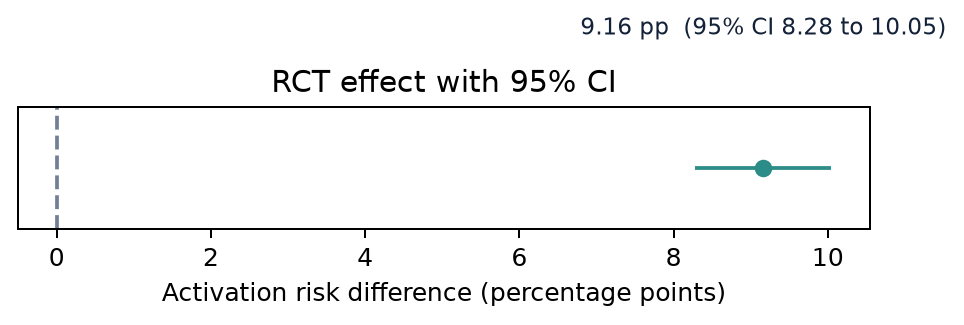
\includegraphics[width=0.9\textwidth]{rct_effect_ci.png}
\tightcaption{Randomized activation effect and confidence interval from the frozen experiment summary.}
\end{figure}

The ITT risk difference is \RiskDifference{} with a 95\% confidence interval of \RiskCI{} and \ExperimentPValue{}. The p-value is reported as a threshold because the stored floating-point value is zero, not because a literal zero probability was established. The interval is far from zero under the stated experiment model, but statistical evidence does not by itself establish profit, durable retention, or external validity.

\begin{table}[!htbp]
\centering
\caption{Experiment guardrails recorded in the frozen run.}
\small
\begin{tabularx}{\textwidth}{@{}Y r r l@{}}
\toprule
Guardrail & Value & Threshold & Status \\
\midrule
\GuardrailRows
\bottomrule
\end{tabularx}
\end{table}

\source{\path{artifacts/results.json}, \path{artifacts/tables/experiment_summary.csv}, \path{artifacts/tables/rct_guardrails.csv}, and \path{docs/experiment_design.md}}

\section{Observational campaign: DiD and IPTW}

The campaign analysis uses a selected-region observational design. Its repeated weekly panel contains \CampaignComparisonN{} comparison customers and \CampaignTreatmentN{} selected-region customers. It reports a difference-in-differences contrast and a stabilized inverse-probability-of-treatment weighted (IPTW) estimate. The unweighted DiD is \CampaignDiD{}; the weighted estimate is \CampaignIPTW{} with standard error \CampaignSE{} and 95\% interval \CampaignIPTWCI{}. The effective sample size is \CampaignESS{} under the recorded uncertainty calculation.

\begin{figure}[!htbp]
\centering
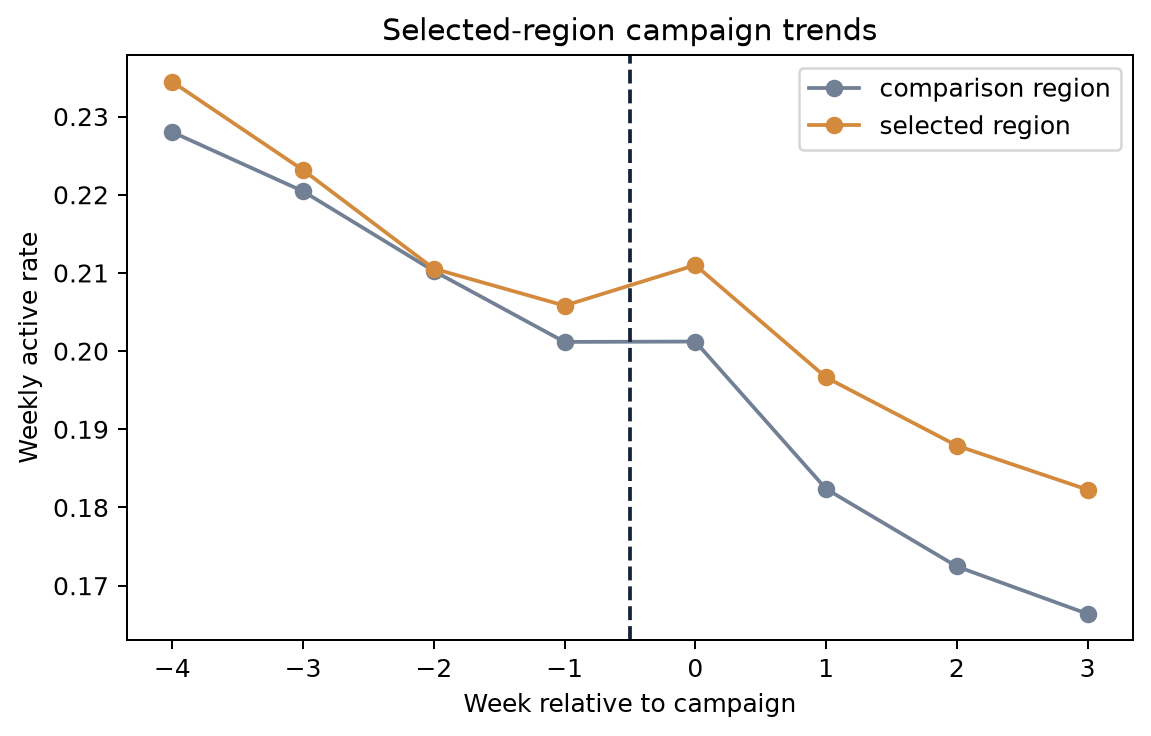
\includegraphics[width=0.86\textwidth]{campaign_weekly_trends.png}
\tightcaption{Weekly activity rates for the selected region and comparison group. The post-period gap is larger than the recorded pre-period gaps.}
\end{figure}

\begin{table}[!htbp]
\centering
\caption{Pre-period and post-period activity rates. Relative week 0 is the first post-period row in the generated table.}
\scriptsize
\begin{tabular}{@{}r r r r@{}}
\toprule
Relative week & Comparison & Selected region & Difference \\
\midrule
\PretrendRows
\bottomrule
\end{tabular}
\end{table}

\subsection{Diagnostics and assumptions}

The common-support diagnostic records \CommonSupport{} and the maximum absolute standardized mean difference after stabilized weighting is \WeightedMaxSMD{}. The unweighted region indicators remain highly imbalanced; weighting reduces measured differences in the recorded covariates. These are diagnostics only. The registry status ``pass'' means the configured diagnostic thresholds passed. It is not causal validation.

The estimate requires parallel untreated trends, no differential contemporaneous shock, stable composition, exchangeability conditional on measured covariates, positivity, correct propensity specification, and no post-treatment features. The stored standard error uses a normal approximation on weighted customer-week means and ignores within-customer correlation. Region assignment is a design feature that must be justified with internal evidence before treating the estimate as causal.

\claim{The campaign result is an observational estimate subject to its assumptions. Measured balance and overlap do not address unmeasured confounding or prove that the campaign caused the post-period difference.}

\section{Churn and response models}

The churn task predicts no meaningful activity in the following 30 days for customers active at the feature cutoff. \SelectionRule{} It is evaluated on a later temporal holdout of \ChurnEvaluationN{} customers. Its ROC AUC is \ChurnAUC{}, top-decile lift is \ChurnLift{}, and top-decile capture is \ChurnCapture{}. The top-decile set contains \ChurnTopDecileN{} customers. These values support a capacity-aware risk ranking under the evaluation sample. They do not estimate treatment benefit.

\begin{table}[!htbp]
\centering
\caption{Churn model comparison on the later temporal holdout.}
\scriptsize
\begin{tabularx}{\textwidth}{@{}Y r r r r r@{}}
\toprule
Model & Brier & ROC AUC & PR AUC & Lift at 10\% & Capture at 10\% \\
\midrule
\ModelRows
\bottomrule
\end{tabularx}
\end{table}

\begin{figure}[!htbp]
\centering
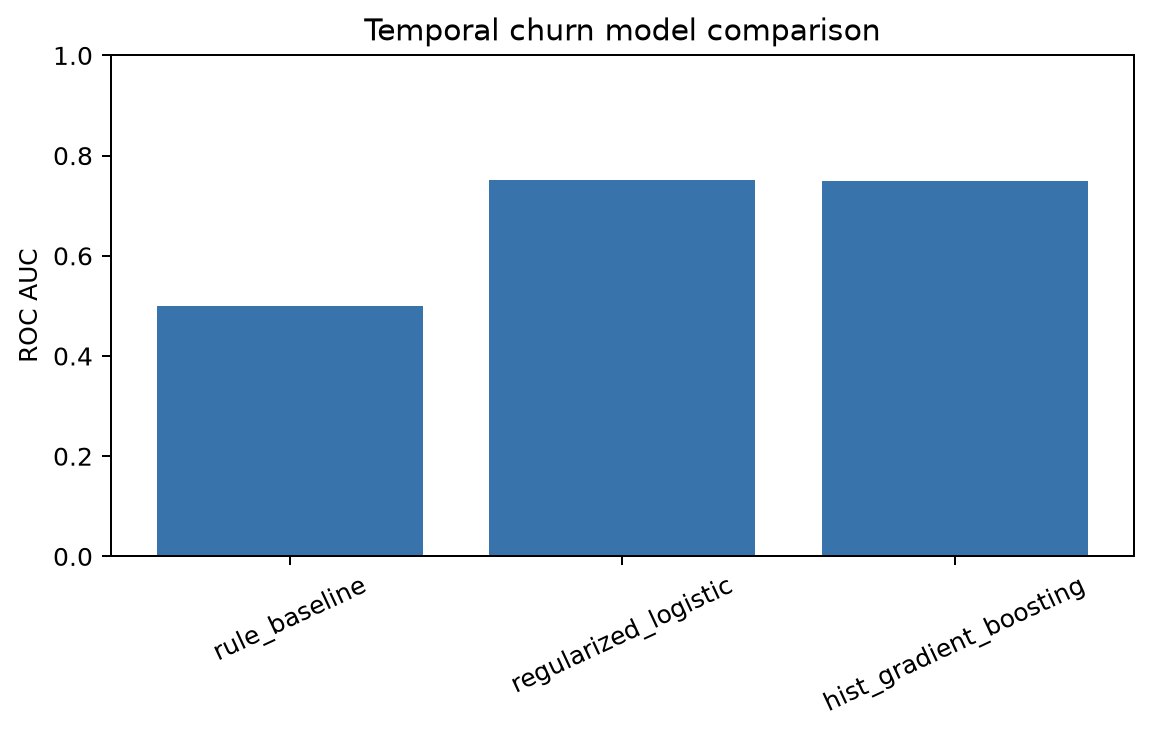
\includegraphics[width=0.47\textwidth]{churn_model_comparison.png}\hfill
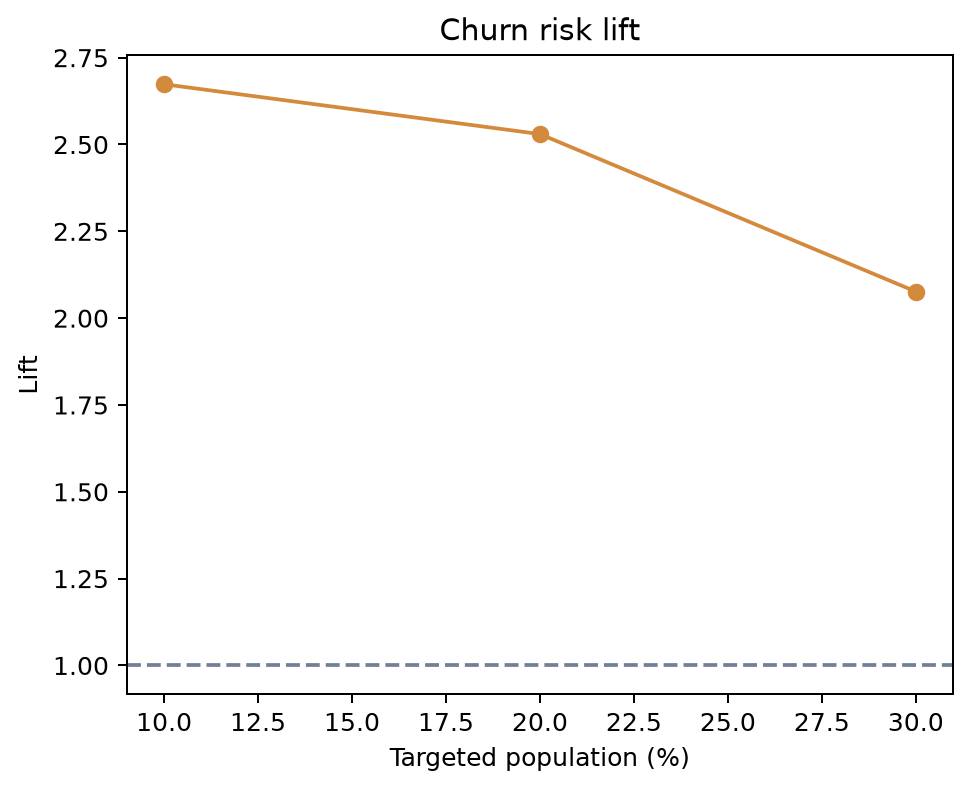
\includegraphics[width=0.47\textwidth]{churn_lift.png}
\tightcaption{Model comparison and concentration of churn events in the scored population.}
\end{figure}

The response propensity model predicts observed activation among treated, eligible customers. It is evaluated on a later temporal holdout of \ResponseEvaluationN{} customers. Its ROC AUC is \ResponseAUC{}, top-decile lift is \ResponseLift{}, and top-decile capture is \ResponseCapture{}. The top-decile set contains \ResponseTopDecileN{} customers. This target is not an uplift estimate: it does not compare each customer's treated and untreated potential outcomes. A contact policy therefore requires incremental response evidence, a holdout design, and harm and cost guardrails.

\begin{figure}[!htbp]
\centering
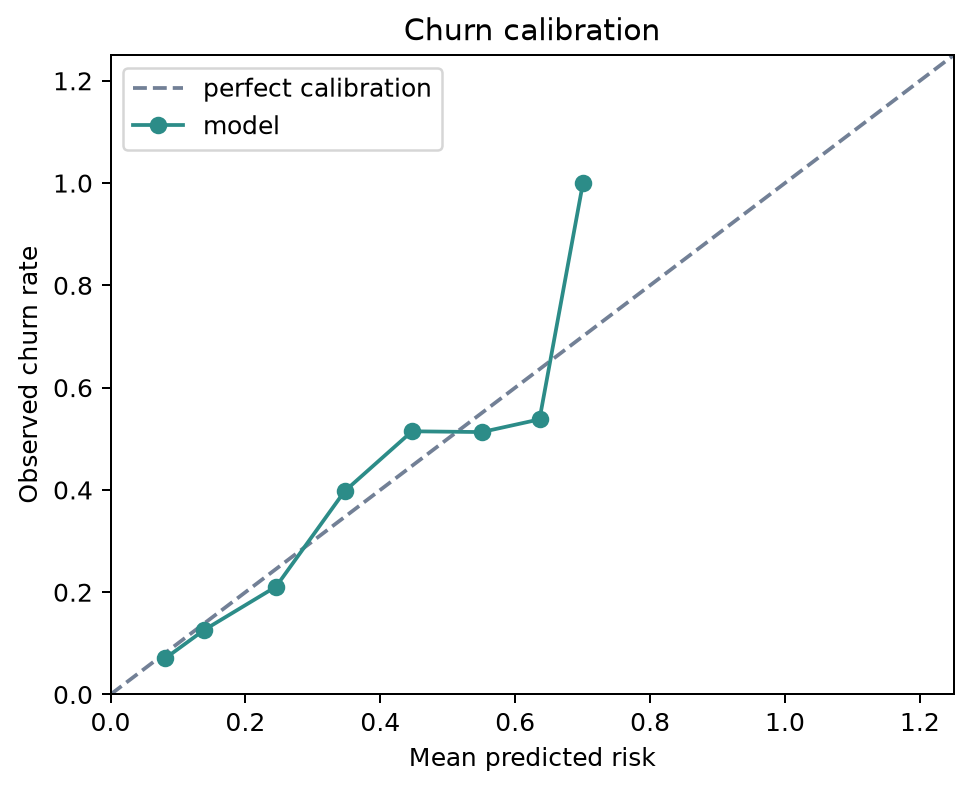
\includegraphics[width=0.7\textwidth]{churn_calibration.png}
\tightcaption{Calibration by predicted-risk bin for the selected churn model. Sparse high-risk bins remain a limitation.}
\end{figure}

\section{Targeting economics}

The economic policy evaluates \EvaluatedPopulation{} customers under explicit fictional assumptions: conditional treatment effect \TreatmentEffectAssumption{}, contact cost \ContactCost{} units, incentive cost \IncentiveCost{} units, and a capacity fraction of \CapacityFraction{}. The strategy table records expected net value under these assumptions.

\begin{figure}[!htbp]
\centering
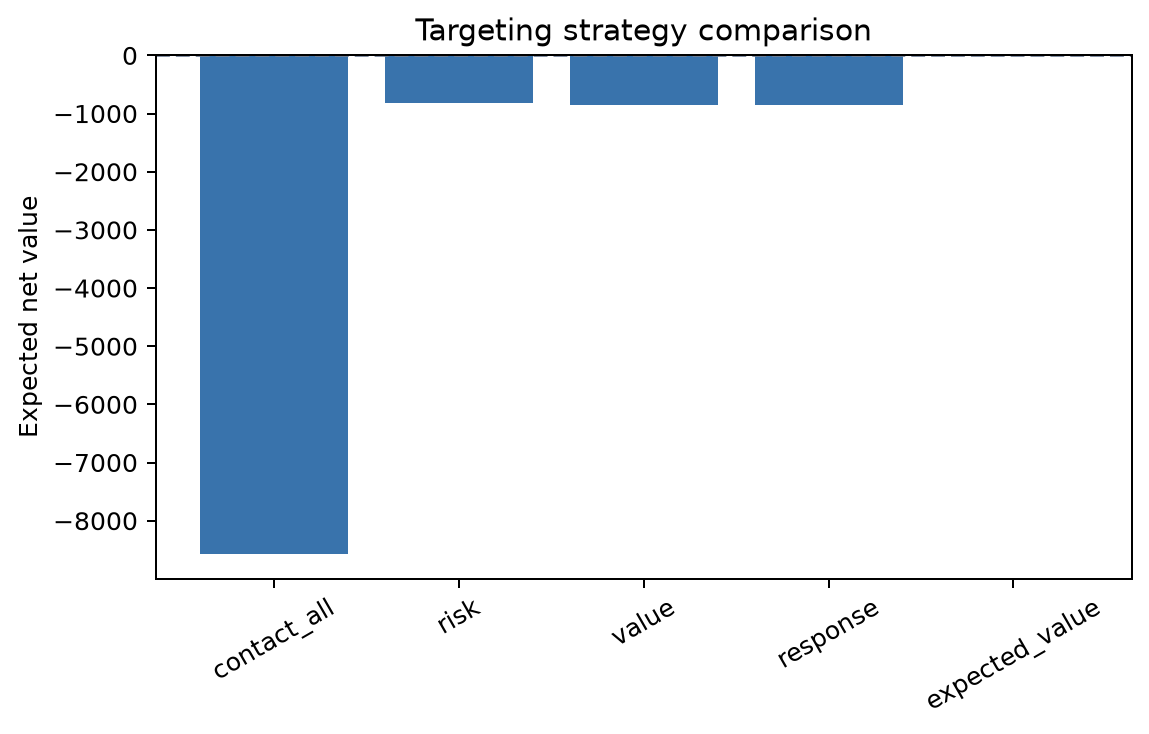
\includegraphics[width=0.84\textwidth]{targeting_strategy_value.png}
\tightcaption{Expected net value by targeting strategy under the recorded scenario assumptions.}
\end{figure}

\begin{table}[!htbp]
\centering
\caption{Targeting strategy comparison. Expected values are fictional units.}
\scriptsize
\begin{tabularx}{\textwidth}{@{}Y r r r l@{}}
\toprule
Strategy & Customers contacted & Contact rate & Expected net value & Profitable \\
\midrule
\EconomicsRows
\bottomrule
\end{tabularx}
\end{table}

The expected-value policy is therefore conservative: it contacts no customers because the estimated value of a positive contact is not sufficient under the scenario. This is a scenario decision, not evidence that all real outreach is unprofitable. The assumptions require internal value, cost, incremental-effect, and capacity inputs before operational use.

\section{Monitoring and temporal stability}

The monitoring artifact reports performance by temporal bucket and feature population stability index (PSI). The maximum feature PSI is \MaxPSI{}, below the configured low-drift reference of 0.1. This is a current synthetic-run diagnostic. It does not establish production stability.

\begin{table}[!htbp]
\centering
\caption{Temporal holdout performance for the selected churn model.}
\scriptsize
\begin{tabularx}{\textwidth}{@{}L{25mm}r r r r r@{}}
\toprule
Time bucket & Customers & Base rate & ROC AUC & Lift at 10\% & Calibration error \\
\midrule
\MonitoringRows
\bottomrule
\end{tabularx}
\end{table}

\begin{figure}[!htbp]
\centering
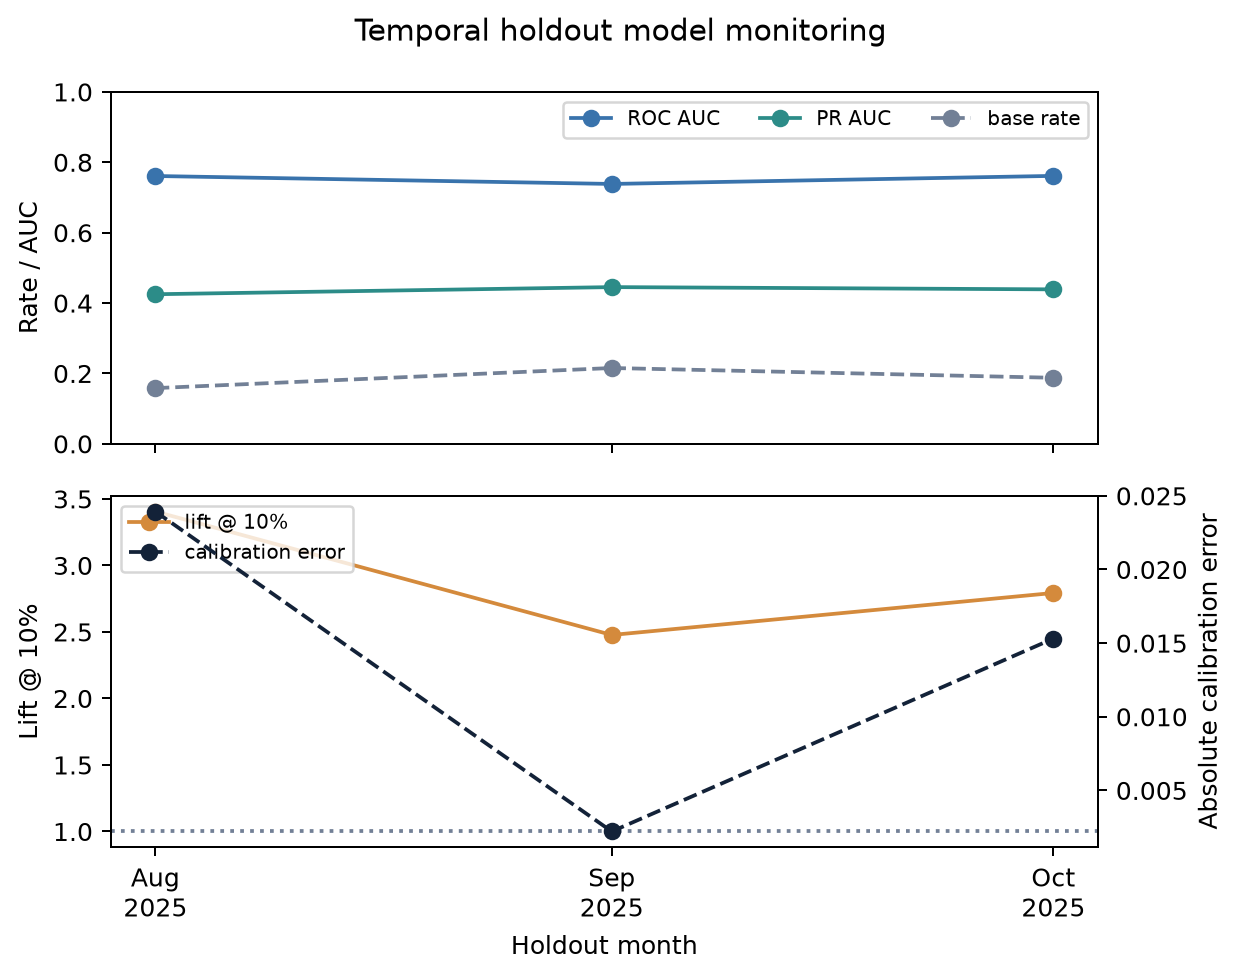
\includegraphics[width=0.78\textwidth]{model_performance_over_time.png}
\tightcaption{Performance over temporal holdout buckets. Monitoring should retain the metric definitions and operating-capacity thresholds used here.}
\end{figure}

The observed bucket variation is material enough to justify continued monitoring, even though the stored status does not indicate recalibration or retraining. A production monitoring plan would need a live data-quality contract, missingness and latency checks, outcome-delay handling, subgroup harm checks, and an approved response to threshold breaches.

\section{Indian-bank directional evidence}

The simulator uses public disclosures from Indian banks to motivate lifecycle heterogeneity. The disclosures describe different units, such as registered users, monthly active users, engagements, digital transaction share, and product adoption. They are not comparable to the Pulse signup-cohort retention windows.

\begin{longtable}{@{}L{25mm}L{17mm}L{64mm}L{38mm}@{}}
\caption{Directional public evidence and design implications. These sources do not provide numerical benchmarks for Pulse retention.}\label{tab:bank-evidence}\\
\toprule
Bank & Period & Evidence recorded in the source registry & Design implication \\
\midrule
\endfirsthead
\toprule
Bank & Period & Evidence recorded in the source registry & Design implication \\
\midrule
\endhead
\BankRows
\bottomrule
\end{longtable}

The evidence supports modeling distinct registered and active states, changing channel mix, product depth, non-primary users, repeat activity, and cohort-level shocks. It does not support setting the synthetic D7, D30, D60, or D90 rates equal to any reported bank metric.

\section{Conclusions and limitations}

The verified results support three limited conclusions. First, the activation experiment records a positive ITT estimate for the eligible synthetic population. Second, the selected-region campaign produces a positive observational contrast, and the configured overlap and balance diagnostics pass, but the causal assumptions remain unverified. Third, the churn ranking is useful as predictive concentration evidence, while response scores and targeting economics do not establish incremental value.

The resulting decision is to keep activation behind controlled experimentation and to withhold positive-contact outreach under the supplied fictional assumptions. The report does not support a production rollout, a claim of customer impact, or a claim that the campaign caused the observed change.

Limitations are structural. The data are behaviorally plausible simulation, not customer data. The simulation's hidden mechanisms can validate selected calculations but do not validate external performance. The observational analysis can remain confounded. Temporal evaluation covers the recorded holdout buckets but cannot forecast policy or population change. Predictive models can drift and can harm subgroups even when aggregate metrics look stable. The economics are assumption-driven. External bank disclosures are directional and use incompatible denominators.

\clearpage
\appendix
\section{Reproducibility and evidence map}

The report is generated in two steps. The evidence generator reads the frozen artifacts and writes a LaTeX include. Tectonic compiles the main source to the requested PDF path.

\begin{verbatim}
make report
\end{verbatim}

The explicit commands are:

\begin{verbatim}
.venv/bin/python scripts/build_latex_inputs.py
tectonic -X compile --outdir reports \
  reports/pulse_case_study.tex
\end{verbatim}

The generator validates required denominators before writing the include. It reconciles the signup and D30 counts, each experiment arm's counts and rate, the randomized effect and interval, campaign group sizes, selected-model and response metrics, holdout populations, and the weighted maximum standardized mean difference across the manifest and detailed tables.

\begin{table}[!htbp]
\centering
\caption{Primary report inputs and their roles.}
\small
\begin{tabularx}{\textwidth}{@{}L{48mm}Y@{}}
\toprule
Artifact & Role in this report \\
\midrule
\path{artifacts/results.json} & Run scope, headline metrics, claim scopes, assumptions, and limitations. \\
\path{artifacts/tables/*.csv} & Journey, cohorts, experiment, guardrails, campaign diagnostics, models, monitoring, and economics rows. \\
\path{artifacts/figures/*.png} & Generated figures embedded without recomputation. \\
\path{config/external_benchmarks.yml} & Directional Indian-bank evidence and source URLs. \\
\path{config/metrics.yml} and \path{docs/metric_definitions.md} & Metric definitions and window contracts. \\
\bottomrule
\end{tabularx}
\end{table}

\section{References}

\begin{enumerate}[label={[\arabic*]},leftmargin=24pt]
\item State Bank of India, \emph{SBI FY25 Analyst Presentation}, slide 46. \href{https://sbi.bank.in/documents/17836/0/SBI\%2BAnalyst\%2BPresentation\%2BQ4FY25.pdf/d496fee6-a237-4328-a5ff-7246e4b736b4?t=1746263845521}{source link}
\item Axis Bank, \emph{Integrated Annual Report 2024--25}, p. 127. \href{https://www.axisbank.com/docs/default-source/annual-reports/for-axis-bank/annual-report-for-the-year-2024-2025.pdf}{source link}
\item HDFC Bank, \emph{Integrated Annual Report 2024--25}, pp. 7 and 140--141. \href{https://www.hdfc.bank.in/content/dam/hdfcbankpws/in/en/pdf/annual-reports/2024-25/HDFC_Bank_Annual_Report_2024_25-310202.pdf}{source link}
\item ICICI Bank, ``iMobile is used by one crore customers from other banks,'' February 2024. \href{https://www.icici.bank.in/about-us/news-room/2024/press-release-icici-banks-imobile-is-used-by-one-crore-customers-from-other-banks}{source link}
\item Kotak Mahindra Bank, \emph{Integrated Annual Report 2024--25}, pp. 9 and 24--25. \href{https://www.kotak.com/bank/mailers/annualreport/documents/Kotak\%20Integrated\%20Annual\%20Report\%202024-25.pdf}{source link}
\end{enumerate}

\end{document}
